\documentclass[12pt]{article}
\usepackage[a4paper]{geometry}
\usepackage[myheadings]{fullpage}
\usepackage{amsmath,amssymb,amsthm, enumitem, hyperref, tabto} 
\usepackage{fancyhdr}
\usepackage{arxiv}
\usepackage{lastpage}
\usepackage{graphicx, wrapfig, subcaption, setspace}
\usepackage[font=small, labelfont=bf]{caption} \usepackage{blindtext}
 \usepackage{blindtext}
\usepackage{url, lipsum}
\usepackage{tgbonum}
\usepackage{amsmath,physics}
\usepackage{authblk}
\usepackage{hyperref}
 \hypersetup{ 
     colorlinks=true, 
     linkcolor=blue, 
     filecolor=blue, 
     citecolor =red,       
     urlcolor=cyan,
     pdftitle={Using Spatial Trees to optimize Food Costs for Lower Wage Families}
     } 
\usepackage[super,compress,sort,numbers]{natbib}
\usepackage{csquotes}
\usepackage{multicol}
%\setlength{\multicolsep}{6.0pt plus 2.0pt minus 1.5pt}% 50% of original values
\usepackage{xcolor}
\usepackage{algpseudocode}
\usepackage{algorithm}
\floatname{algorithm}{Algorithm}
\usepackage{times}
\usepackage{adjustbox}
\usepackage[T1]{fontenc}
\usepackage{makecell}
\usepackage{parskip}
\usepackage{erewhon}
\usepackage{geometry}
\usepackage{caption}
\usepackage{subcaption}
\usepackage{framed}
\setlength\FrameSep{0.5em}
\setlength\OuterFrameSep{\partopsep}
% \usepackage{draftwatermark}
\graphicspath{ {./images/} }
\usepackage{sectsty}

\sectionfont{\fontsize{15}{20}\selectfont}
\usepackage{tikz}
\def\checkmark{\tikz\fill[scale=0.4](0,.35) -- (.25,0) -- (1,.7) -- (.25,.15) -- cycle;} 
\usepackage[sorting=none]{biblatex}
\addbibresource{references.bib}

\newcommand{\HRule}[1]{\rule{\linewidth}{#1}}
\onehalfspacing
\setcounter{tocdepth}{5}
\setcounter{secnumdepth}{5}

\renewcommand{\headrulewidth}{0pt}
\renewcommand{\footrulewidth}{0pt}

\begin{document}


\pagestyle{fancy}
\fancyhf{}
\fancyhead[L]{\footnotesize \textbf{CS5132} PA2 - \emph{Using Spatial Trees to optimize Food Costs for Lower Wage Families} }

\fancyfoot[R]{Page \thepage\ of \pageref{LastPage}}


{\selectfont
\title{
	\huge \textbf{Using Spatial Trees to optimize Food Costs for Lower Wage Families}
}

\date{}

\author[1]{Kannan Vishal}
\author[1]{Prannaya Gupta}
\author[1]{Quek Yu Pin}
\author[1]{Vikram Ramanathan}
\affil[1]{NUS High School of Math and Science}

\maketitle

\vspace{-2cm}

\tableofcontents

\thispagestyle{empty}
\newpage

\section{Background}

Lower income families are largely plagued by food expenses nowadays, with it making up a significant proportion of their monthly expenditures. Usually, selection of stores to go to for groceries and meals is largely predicated by convenience of distance, e.g. going to the nearest \textit{7-Eleven}. On the other hand, walking a bit further to the closest \textit{FairPrice} is considered another option over other nearby sources that tend to mark up their products. But what if such families enter a neighbourhood they are unfamiliar with? How can they be sure that they can get meals for affordable prices? In this study, we intend to prepare a platform to present such options in a relatively concise interfaces, that allows selection based on \textbf{both price and distance}. This selection is done via the use of Spatial R-Trees and QuadTrees.


This way, users can make more informed decisions on their food expenditures.
    
   
\section{User Documentation}
You are to provide a brief user documentation with \textbf{screenshots} on how to use the
program and its functionalities.

\section{Analysis and Explanation of Implemented Tree Methods}

Provide a brief explanation, in your own words, and rigorous mathematical worst-case
analysis derivation and time complexity of the key methods of your tree structure
(retrieval, insertion, deletion, balance (if any))



\subsection{Spatial Quad-Trees}
\begin{figure}
    \centering
    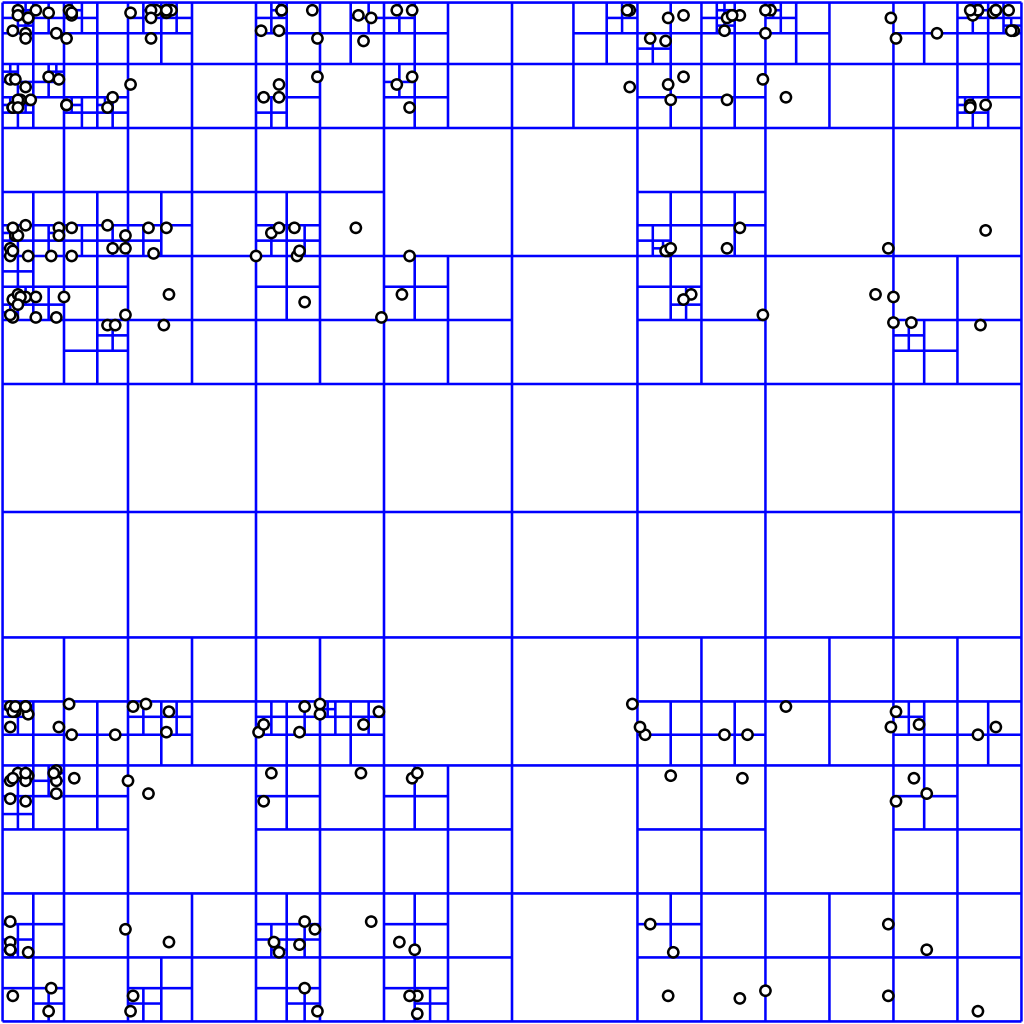
\includegraphics[scale=0.3]{../img/quadtree.png}
    \caption{Quad-Tree visualization}
    \label{fig:my_label}
\end{figure}
Quad-Trees are commonly used in analysing the distribution of a collection in 2D space, as the size and precision of the data structure scales with the distribution of the spatial data we are working with. As we map out store branches over Singapore, we may find that the locations are not evenly distributed. If we try to split up the map of Singapore into a grid, and check if each grid is occupied by a store, then we may have a lot of overlap of stores in shopping districts, and wasted space in more residential areas. 

Quad-Trees address this by also splitting up the map into four quadrants and recursively making quadrants within those quadrants, but lazily. That is, a quadrant is subdivided only during when there is a child node to be inserted into the quadrant. The depth of the tree is thus proportional to the density of points, which results in many speedups.

\subsubsection{Algorithm}

In terms of implementation, Quad-Trees are essentially binary search trees where the internal nodes have degree four instead of two. 

\subsection{Spatial R-Trees}

\begin{figure}
    \centering
    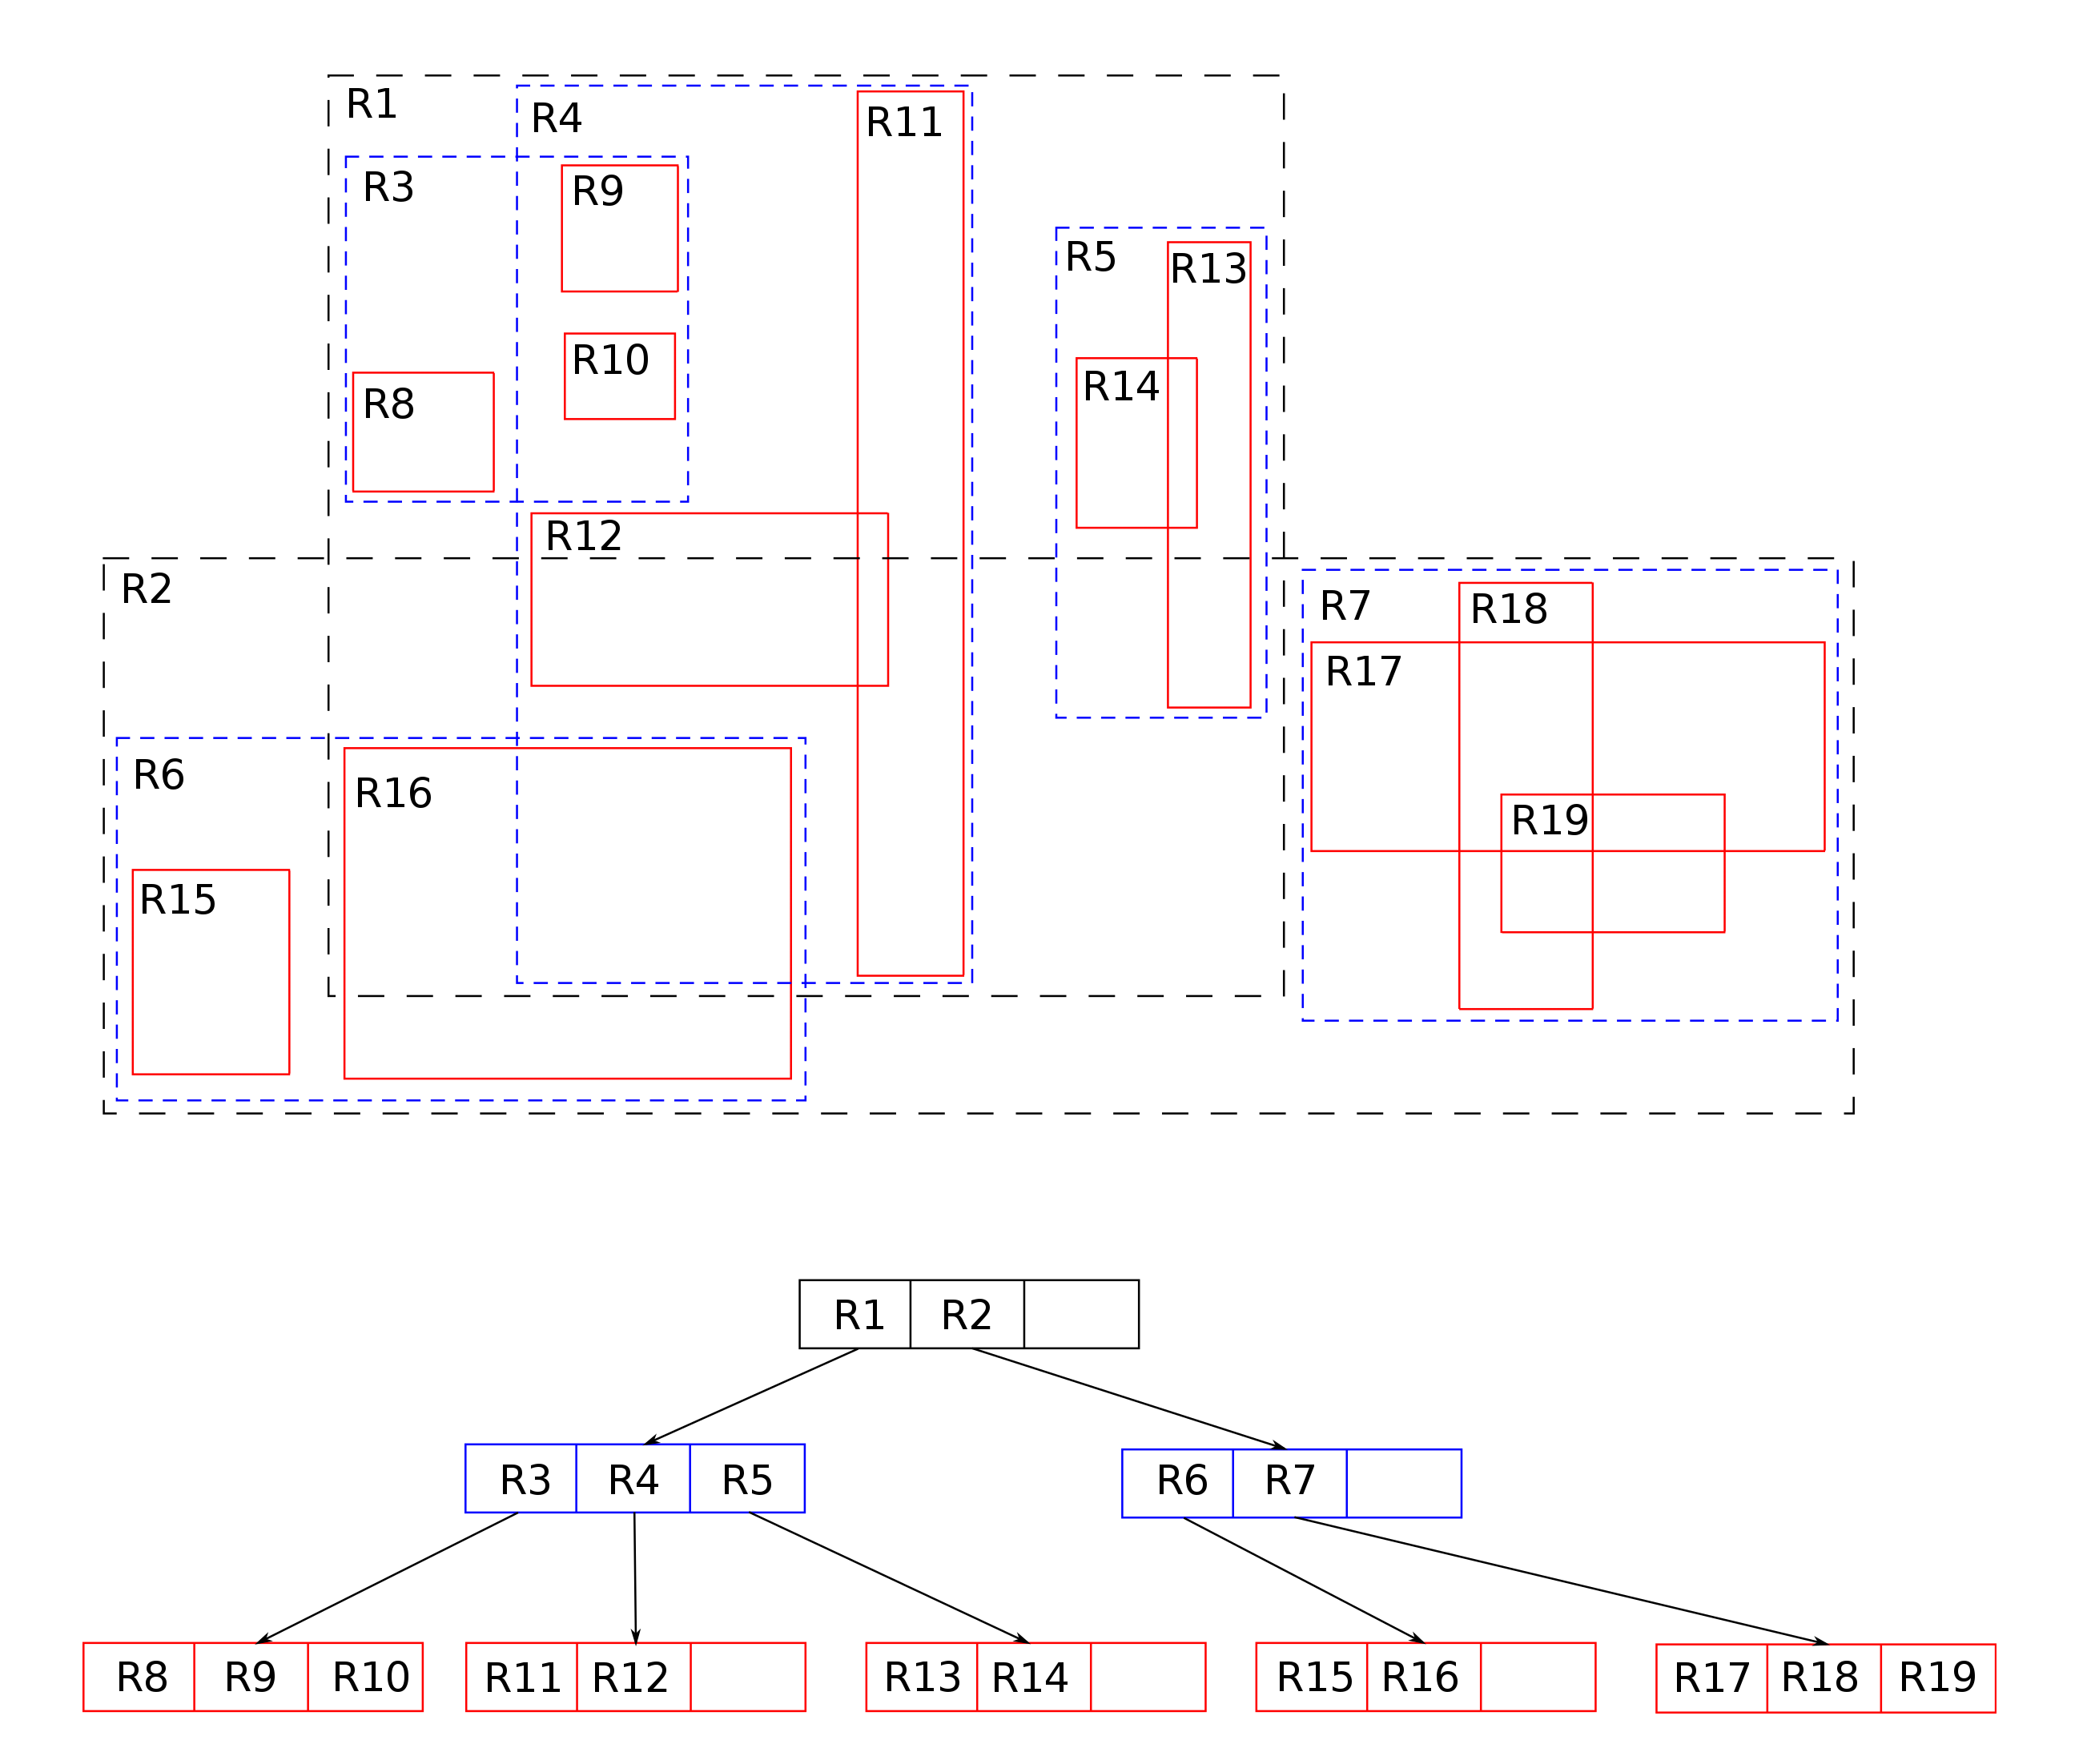
\includegraphics[scale=0.3]{../img/RTree.png}
    \caption{R-Tree visualization}
    \label{fig:my_label}
\end{figure}

Another approach to storing points in space, especially for our purposes of nearest neighbour queries, is to group points together, according to their closeness, and then recursively group those groups together. 

\subsubsection{Algorithm}



\subsection{R-Trees vs. Quad-Trees}

% Hypothesis
% Why we think one would work better

\section{Testing Strategy}
You are to provide at least \textbf{3 test cases} you used to test the correctness and
robustness of your program. Log down the sample input and output for each test case.
Briefly explain why each test case was chosen.



\section{Results}

% Which data structure did better

\newpage
\section{GitHub Information}
You can find our repository at \url{https://github.com/ThePyProgrammer/SnackNow}.

\subsection{User Directory}
\begin{center}
    \begin{tabular}{|c|c|}
        \hline
        GitHub Username & Real Name \\
        \hline
        \href{https://github.com/delargement}{\texttt{delargement}} & Kannan Vishal \\
        \href{https://github.com/ThePyProgrammer}{\texttt{ThePyProgrammer}} & Prannaya Gupta \\
        \href{https://github.com/h1810126}{\texttt{h1810126}} & Quek Yu Pin \\
        \href{https://github.com/VikramRamanathan}{\texttt{VikramRamanathan}} & Vikram Ramanathan \\
        \hline
    \end{tabular}
\end{center}


\subsection{Repo Report}

\section{Reflection}

\subsection{Vishal}

By helping out a here and there in each component of the project, and reviewing our project while writing the report, I have gained a better understanding of the software development lifecycle, from the brainstorming stage, UI prototyping stage, data collection and documentation. By abstracting each component of the project, such as the model (RTree and Quadtree implementation) and GUI, and distributing the workload, we were able to be more productive, and it was enjoyable to see each of the pieces to connect together to give a minimum viable product.

\subsection{Prannaya}

\subsection{Yu Pin}

\subsection{Vikram}

\section{Work Distribution Matrix}

\begin{center}
\begin{tabular}{|c|c|c|c|c|}
    \hline
    & Vishal & Prannaya & Yu Pin & Vikram \\ [0.5ex] 
    \hline\hline
    Ideation & &  &  & \checkmark \\
    R-Tree Implementation &  & \checkmark &  &  \\
    Quad-Tree Implementation &  &  &  & \checkmark \\
    Data Collection &  &  & \checkmark &  \\
    User Interface  & \checkmark & \checkmark &  &  \\
    Report  & \checkmark & \checkmark  &  &  \\
    \hline
\end{tabular}
\end{center}


\newpage


\section{References}

\printbibliography[
heading=none
]
}

\end{document}